\documentclass[12pt, letterpaper]{article}
\usepackage[top=2.5cm, bottom=2.5cm, left=3cm, right=2.5cm]{geometry}
\usepackage[utf8]{inputenc}
\usepackage[T1]{fontenc}
\usepackage{lmodern}
\usepackage{amsmath, amssymb}
\usepackage{booktabs}
\usepackage{tabularx}
\usepackage{longtable}
\usepackage{array}
\usepackage{multirow}
\usepackage{xcolor}
\usepackage{graphicx}
\usepackage{float}
\usepackage{listings}
\usepackage[most, breakable]{tcolorbox}
\usepackage{enumitem}
\usepackage{fancyhdr}
\usepackage{titlesec}
\usepackage{setspace}
\usepackage{microtype}
\usepackage[hidelinks]{hyperref}
\usepackage{parskip}
\usepackage{pgfplots}
\usepackage{xcolor}
\pgfplotsset{compat=1.15}
\usepackage{tikz}
\usetikzlibrary{arrows.meta,positioning}
% Define textbook colors
\definecolor{beteal}{RGB}{0,120,120}
\definecolor{beblue}{RGB}{40,80,160}
\definecolor{berust}{RGB}{170,70,40}
\definecolor{bepurple}{RGB}{100,60,150}
% Colours
\definecolor{econblue}{RGB}{31,78,121}
\definecolor{researchgreen}{RGB}{21,101,45}
\definecolor{exampleorange}{RGB}{180,80,20}
\definecolor{lightgray}{RGB}{245,245,245}
\definecolor{boxblue}{RGB}{220,235,248}

% Section headings
\titleformat{\section}{\large\bfseries\color{econblue}}{\thesection}{1em}{}%
  [\vspace{-4pt}\rule{\linewidth}{0.4pt}]
\titleformat{\subsection}{\normalsize\bfseries\color{econblue}}{\thesubsection}{1em}{}
\titleformat{\subsubsection}{\normalsize\bfseries}{\thesubsubsection}{1em}{}

% Page style
\pagestyle{fancy}
\fancyhf{}
\fancyhead[L]{\small\itshape ECON 230 --- Introduction to Behavioural Economics}
\fancyhead[R]{\small\itshape Chapter 5: Why We Don't Save Enough}
\fancyfoot[C]{\small\thepage}
\renewcommand{\headrulewidth}{0.4pt}
\setlength{\headheight}{14pt}

% tcolorbox styles
\tcbuselibrary{breakable, skins, listings}

\newtcolorbox{researchbox}{
  enhanced, breakable,
  colback=researchgreen!6, colframe=researchgreen!55,
  title=\textbf{Research Study},
  fonttitle=\bfseries\small,
  attach boxed title to top left={yshift=-2mm, xshift=6mm},
  boxed title style={colback=researchgreen!55, colframe=researchgreen!55},
  before upper={\setlength{\parskip}{4pt}}
}

\newtcolorbox{examplebox}[1]{
  enhanced, breakable,
  colback=exampleorange!6, colframe=exampleorange!45,
  title=\textbf{#1}, fonttitle=\bfseries\small
}

\newtcolorbox{keybox}{
  enhanced, colback=boxblue, colframe=econblue!70,
  fontupper=\small
}

% ASCII figure style
\lstset{
  basicstyle=\scriptsize\ttfamily,
  breaklines=false,
  keepspaces=true,
  columns=flexible,
  frame=single,
  backgroundcolor=\color{lightgray},
  xleftmargin=4pt, xrightmargin=4pt,
  aboveskip=6pt, belowskip=6pt
}

% Lists
\setlist[itemize]{leftmargin=1.5em, itemsep=2pt, topsep=4pt}
\setlist[enumerate]{leftmargin=1.5em, itemsep=2pt, topsep=4pt}
\onehalfspacing

\newcolumntype{Y}{>{\raggedright\arraybackslash}X}

\begin{document}

\begin{titlepage}
\centering\vspace*{3cm}
{\Large\bfseries\color{econblue} ECON 230 --- Introduction to Behavioural Economics\\[1em]}
{\large\bfseries Course Textbook\\[2em]}
{\LARGE\bfseries\color{econblue} Chapter 5\\[0.5em]}
{\Large\bfseries Why We Don't Save Enough --- Behavioural Approaches to Savings\\[2em]}
\vfill
{\normalsize University of Northern British Columbia\\
Instructor: Prof.\ Muhebullah Karimzada\\
Term: Winter 2027}
\end{titlepage}
\tableofcontents
\newpage


\medskip


\section*{Chapter Overview}
\addcontentsline{toc}{section}{Chapter Overview}


Chapter 4 established the theoretical mechanism behind undersaving: present bias, represented formally by the $\beta$-$\delta$ model, causes agents to systematically prefer immediate consumption over future provision, generating a persistent gap between savings intentions and savings behaviour. This chapter takes the analysis from the abstract to the concrete. It examines \textit{how} present bias, combined with several additional behavioural forces, manifests in actual household savings decisions --- and what evidence-based interventions can do about it.

The chapter opens by revisiting the life-cycle model of savings, the benchmark from standard economics, and cataloguing its specific failures. It then introduces \textbf{mental accounting} --- the tendency to categorise money into distinct psychological "buckets" with different spending norms --- as a second major force shaping savings behaviour, complementary to but distinct from present bias. Mental accounting helps explain one of the most striking puzzles in household finance: why millions of households simultaneously hold high-interest credit card debt and low-interest savings, when paying down the debt would be a risk-free windfall.

The chapter examines the \textbf{sunk cost fallacy} --- the irrational attention to past, irretrievable costs --- as a related feature of mental accounting. It develops the \textbf{compound interest illusion}: the systematic human tendency to underestimate exponential growth, with large consequences for retirement savings. It then presents the \textbf{minimum payment trap} --- a behavioural phenomenon in credit markets with particularly severe consequences for lower-income households --- alongside the regulatory response the Government of Canada adopted.

The second half of the chapter turns to solutions: the powerful evidence on \textbf{automatic enrolment defaults} (Madrian and Shea, 2001), the role of \textbf{financial literacy} and its surprising limits, and the design principles that make savings interventions effective. Throughout, the Canadian institutional context --- the RRSP, the TFSA, the CPP, and the evolving policy landscape --- anchors the analysis in the settings most relevant to students.

\medskip


\section*{Learning Objectives}
\addcontentsline{toc}{section}{Learning Objectives}


After studying this chapter, students should be able to:

\begin{enumerate}
\item \textbf{Explain} the life-cycle hypothesis (LCH) of savings, state its four key predictions, and identify the specific empirical failures of each prediction.
\item \textbf{Define} excess sensitivity of consumption and explain why it violates the LCH, using evidence from tax refunds and predictable income changes.
\item \textbf{Define} mental accounting, explain the three-account model (Shefrin and Thaler, 1988), and explain why money is not treated as fungible across accounts.
\item \textbf{Explain} the sunk cost fallacy, identify it in real economic decisions, and explain why it constitutes a departure from rational choice.
\item \textbf{Describe} the debt-savings paradox --- households holding high-interest debt and low-return savings simultaneously --- and explain it using mental accounting.
\item \textbf{Define} the compound interest illusion and explain why linear thinking about exponential processes leads to systematic underestimation of long-run savings growth.
\item \textbf{Analyse} the minimum payment trap on credit card debt, calculate the total interest cost of minimum payment strategies, and explain the psychological mechanisms that sustain it.
\item \textbf{Explain} the default effect in savings enrolment, describe the Madrian and Shea (2001) study, and assess the evidence for automatic enrolment as a savings policy.
\item \textbf{Assess} the evidence on financial literacy as a policy tool, explaining both why it matters and why it is insufficient on its own.
\item \textbf{Evaluate} the Canadian retirement savings landscape (RRSP, TFSA, CPP) from a behavioural economics perspective, identifying where each instrument succeeds and where it falls short.
\end{enumerate}

\medskip


\section*{Introduction: Is a Dollar Always a Dollar?}
\addcontentsline{toc}{section}{Introduction: Is a Dollar Always a Dollar?}


Before reading further, consider three scenarios and ask yourself how you would respond to each.

\textbf{Scenario A.} You have just won \$5,000 in a provincial lottery scratch ticket.

\textbf{Scenario B.} You received a \$5,000 tax refund from the Canada Revenue Agency.

\textbf{Scenario C.} Your employer gave you a \$5,000 year-end bonus.

In each case, you now have \$5,000 more than you had before. Standard economics says your response should be identical across all three scenarios: \$5,000 is \$5,000. A rational agent with a given set of preferences for present and future consumption should increase savings by the same fraction --- and spend the same fraction --- regardless of which envelope the money arrived in.

But research consistently shows that people do \textit{not} respond identically. Lottery winnings tend to be spent quickly and freely --- the money feels like "found" money, detached from normal budgeting. Tax refunds generate a mix of spending and saving --- the money is perceived as a return of something that was "owed," producing a more serious financial attitude. Year-end bonuses tend to be saved at higher rates --- framed as compensation for professional performance, they feel more like wealth than like windfall.

These differences in response to economically identical windfalls are not random. They are systematic, predictable, and consequential. They reflect a phenomenon called \textbf{mental accounting} --- one of the central subjects of this chapter.

The same phenomenon that treats lottery winnings and bonuses differently also underlies the savings crisis that Canada, in common with most rich countries, is experiencing. Understanding why Canadians do not save enough --- and what can realistically be done about it --- requires understanding not just present bias (Chapter 4) but the full set of behavioural forces that shape intertemporal financial decisions.

\medskip


\section{The Life-Cycle Hypothesis: The Benchmark and Its Failures}



\subsection{The Model}


The standard economic theory of household savings is the \textbf{life-cycle hypothesis (LCH)}, developed by Franco Modigliani and Richard Brumberg in 1954, building on Milton Friedman's related \textbf{permanent income hypothesis} (1957). Modigliani was awarded the Nobel Memorial Prize in Economics in 1985, in part for this contribution.

The core idea is elegant: a rational, time-consistent agent plans their consumption over their entire lifetime. In young adult years, income is typically low relative to anticipated lifetime earnings, so the agent borrows to support consumption. In prime working years, income is high and the agent saves --- accumulating the wealth that will support retirement consumption. In retirement, income from work falls to zero and the agent draws down the accumulated savings.

This pattern --- borrow young, save in prime years, dissave in retirement --- is called \textbf{consumption smoothing}: the agent allocates resources across time to maintain a relatively stable standard of living rather than experiencing dramatic swings in consumption as income fluctuates.

\textbf{The Four Key Predictions of the LCH:}

\textbf{Prediction 1: Low marginal propensity to consume (MPC) from temporary income shocks.} If a worker receives an unexpected one-time payment of \$10,000 and has 20 remaining years of life, the LCH predicts they will spread this windfall evenly across those 20 years, consuming only \$500 per year more --- an MPC of approximately 5\%. The other 95\% is saved.

\textbf{Prediction 2: No response to predictable income changes.} If an agent knows their income will rise in January (a scheduled raise) or that they will receive a tax refund in March, that information was already incorporated into their lifetime plan when formed. The actual arrival of the income should generate no additional spending --- it was already "spent" in the plan.

\textbf{Prediction 3: Dissaving in retirement.} Retirees should draw down their wealth during retirement, consuming more than their current (pension) income and dying with approximately zero net assets (or a planned bequest if they have altruistic preferences toward heirs).

\textbf{Prediction 4: Consumption smoothing across the life cycle.} Consumption should be roughly flat across the lifecycle (or smoothly rising if income growth is expected), with no sharp drops or spikes corresponding to income changes.

\textbf{Figure 5.1: The Life-Cycle Model}
\begin{figure}[h]
\centering

\begin{tikzpicture}

\begin{axis}[
    width=0.9\textwidth,
    height=0.45\textheight,
    xlabel={Age},
    ylabel={Income, Consumption, Net Saving},
    xmin=20,
    xmax=85,
    ymin=-60,
    ymax=120,
    axis lines=left,
    title={Life Cycle: Income, Consumption \& Net Savings},
    xtick={20,30,40,50,60,70,80},
    ytick={-50,0,50,100},
    clip=false,
    tick label style={font=\small},
    label style={font=\small},
    title style={font=\small},
    legend style={
        at={(0.5,-0.18)},
        anchor=north,
        font=\small,
        legend columns=3
    }
]

% Income profile
\addplot[
    beteal,
    very thick,
    domain=20:80,
    samples=150
]
{100*sin(deg((x-20)*pi/60))*0.9+10};

% Consumption (smooth constant)
\addplot[
    beblue,
    very thick,
    domain=20:80
]
{55};

% Net saving
\addplot[
    berust,
    dashed,
    thick,
    domain=20:80,
    samples=150
]
{100*sin(deg((x-20)*pi/60))*0.9+10-55};


% Zero saving line
\draw[
    gray,
    dashed,
    thin
]
(axis cs:20,0) -- (axis cs:80,0);


% Labels (placed away from curves)
\node[
    font=\small,
    beteal,
    anchor=west
]
at (axis cs:56,100)
{Income};

\node[
    font=\small,
    beblue,
    anchor=west
]
at (axis cs:69,60)
{Consumption};

\node[
    font=\small,
    berust,
    anchor=west
]
at (axis cs:67,15)
{Net Saving};


% Borrowing annotation
\node[
    font=\small,
    align=center,
    berust
]
at (axis cs:30,-35)
{\textit{Borrowing}\\region};


\legend{
Income,
Consumption,
Net Saving
}

\end{axis}

\end{tikzpicture}

\caption{A standard life-cycle model: income rises and falls over working life, consumption is smoothed, and saving is positive during peak earnings years and negative when young or retired.}

\end{figure}



\begin{table}[H]
\centering
\small
\begin{tabularx}{\linewidth}{lY}
\toprule
 & Description \\
\midrule
\textbf{What the figure shows} & Three curves plotted against age (horizontal axis, roughly 20--80). The income curve rises from age 20, peaks around age 50--55, then falls sharply to a low level at retirement. The consumption curve is approximately flat --- smoothed across the life cycle. The net savings curve (income minus consumption) is negative in youth (borrowing), positive and rising in prime working years (saving), and negative again in retirement (dissaving). \\
\textbf{How to interpret it} & The LCH predicts that consumption is not constrained by current income but by lifetime income, with savings acting as the buffer that allows consumption to be smooth. Large divergences between current income and consumption --- borrowing in youth, large savings in prime years, large dissaving in retirement --- are the model's central prediction. The empirical evidence contradicts several of these predictions. \\
\bottomrule
\end{tabularx}
\end{table}



\subsection{The Four Failures of the LCH}


\textbf{Failure 1: Excess sensitivity.} Consumption is far more sensitive to current income than the LCH predicts. Flavin (1981) and subsequent researchers showed that consumption responds strongly to predictable income changes --- changes that rational agents should have already incorporated in their plans. A scheduled pay raise raises consumption immediately rather than being smoothed backward into prior periods.

The most compelling Canadian illustration is the response to tax refunds. The Canada Revenue Agency issues approximately 18 million income tax refunds each year, with an average refund of approximately \$1,895. The LCH predicts that the average recipient would spend only about \$95 of this refund in the year it arrives (roughly 5\%, spread over a 20-year consumption horizon). Studies of actual consumer spending find that Canadians increase spending by 25--50\% of their refund in the month it arrives --- a response 5 to 10 times larger than the LCH predicts. Retailers with Canadian operations --- including Canadian Tire, Best Buy, and Walmart --- have long exploited this, running "Tax Refund Events" in February and March and documenting 15--20\% sales spikes that coincide precisely with the CRA's refund schedule.

Souleles (1999) documented the same excess sensitivity for US Social Security payments. Consumption rose sharply when Social Security cheques arrived --- even though the timing was entirely predictable months in advance and should have generated no revision to consumption plans under the LCH. The arrival of the physical cheque, not the information it conveyed, triggered the spending response.

\textbf{Failure 2: The retirement consumption drop.} The LCH predicts consumption should be smooth through retirement. The empirical evidence shows a sharp, significant drop in consumption at retirement --- sometimes called the \textbf{retirement consumption puzzle}. Banks and colleagues (2012) documented a drop of approximately 25--30\% in UK households' non-durable consumption at retirement. Bernheim, Skinner, and Weinberg (2001) found a similar pattern in the United States.

This drop is inconsistent with the LCH if agents knew in advance when they would retire (which they generally do). The standard behavioural explanation is that retirement arrives while savings are insufficient --- households undersaved during their working years due to present bias, and the retirement income drop represents the consequence of that undersaving rather than a planned feature of the lifecycle consumption path.

\textbf{Failure 3: Inadequate dissaving in retirement.} The LCH predicts that retirees should draw down their wealth, spending more than their pension income and dying with approximately zero assets. In practice, many retirees maintain or even increase their wealth in early retirement years, spending far less than their income. This "retirement saving puzzle" (De Nardi, French, and Jones, 2010) partly reflects precautionary saving for uncertain medical costs and uncertain longevity, but also reflects the mental accounting pattern in which accumulated wealth is mentally coded as untouchable capital.

\textbf{Failure 4: Low savings rates.} The LCH predicts savings rates during prime working years should be substantial --- in the range of 15--25\% for many households to adequately fund retirement. As documented in Chapter 4, actual Canadian household savings rates have fallen from over 20\% in 1982 to approximately 5--6\% today. A large fraction of Canadian households will reach retirement with savings inadequate to maintain their working-life standard of living.

\textbf{Table 5.1: Life-Cycle Hypothesis Predictions versus Evidence}


\begin{table}[H]
\centering
\small
\begin{tabularx}{\linewidth}{lYY}
\toprule
LCH Prediction & Empirical Finding & Magnitude of Failure \\
\midrule
MPC from temporary windfall $\approx$ 5\% & Actual MPC $\approx$ 25--50\% of windfall in arrival month & 5--10$\times$ predicted \\
No response to predictable income & Sharp spending spikes at tax refund, payroll, Social Security & Systematic violation \\
Consumption smooth through retirement & ~25\% drop in consumption at retirement & Large and consistent \\
Adequate dissaving in retirement & Many retirees maintain or increase wealth & Opposite of prediction \\
High prime-age savings rate & Canadian savings rate ~5--6\% & Well below needed \\
\bottomrule
\end{tabularx}
\end{table}


\medskip


\section{Mental Accounting}



\subsection{The Core Concept}


\textbf{Mental accounting} is the set of cognitive operations that individuals use to organise, evaluate, and keep track of financial activities (Thaler, 1985, 1999). The fundamental insight is that people do not treat money as perfectly \textbf{fungible} --- interchangeable regardless of its source, form, or intended purpose. Instead, they assign money to distinct mental categories ("accounts"), each with its own set of norms governing how freely the money can be spent.

This is not how rational agents should behave. Money is money: a dollar in a current account, a dollar in a retirement fund, and a dollar received as a gift are equally capable of purchasing the same goods and services. A rational agent would evaluate all dollars on the same scale and allocate them according to a unified set of preferences. Mental accounting violates this by attaching different spending norms to money depending on which psychological "bucket" it belongs to.

Mental accounting was developed by Richard Thaler, building on insights from Kahneman and Tversky's Prospect Theory. Its connection to loss aversion is direct: crossing from one mental account to another can feel like a loss (withdrawing from savings feels like losing savings), even when the rational consequence is an identical financial position.


\subsection{The Three-Account Model}


Shefrin and Thaler (1988) proposed that households maintain three broad mental accounts, each with a characteristic marginal propensity to consume (MPC) --- the fraction of funds in that account that is spent rather than saved:

\textbf{Account 1: Current Income.} This account contains wages, salaries, and other regular income. The MPC from current income is high --- most of what arrives in this account is available for immediate spending. Conventional framing of this money as "this month's budget" establishes an implicit permission to spend it freely.

\textbf{Account 2: Current Assets.} This account contains liquid savings --- funds in chequing and savings accounts, bonds, stocks, home equity lines of credit. The MPC is moderate --- these funds are accessible but spending them feels like a sacrifice (crossing the "boundary" of a savings account). People experience withdrawing from savings as a loss, consistent with loss aversion.

\textbf{Account 3: Future Income.} This account contains funds earmarked for future purposes --- retirement savings (RRSP, pension plans), funds locked in long-term investments, home equity beyond the credit line. The MPC from this account is very low, approaching zero. The mental norm associated with these funds is "don't touch" --- spending them feels like a large loss and a violation of the purpose for which they were intended.

\newpage
\textbf{Figure 5.2: The Three-Account Structure}

\begin{figure}[ht]
\centering

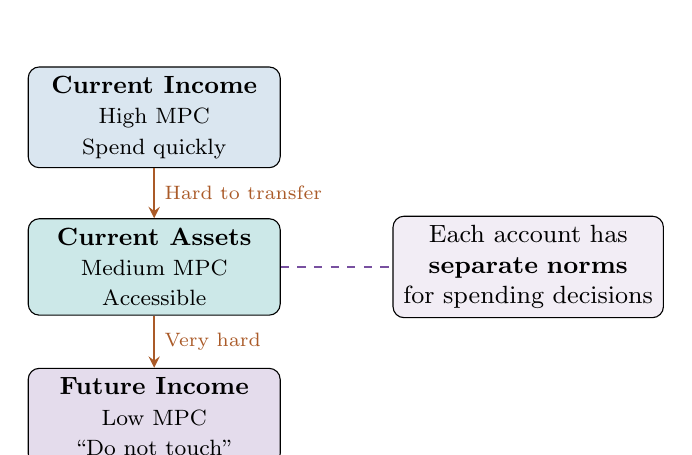
\begin{tikzpicture}[
    scale=0.95,
    node distance=1.2cm,
    >=stealth
]

% Define colours if not already defined
\definecolor{beblue}{RGB}{70,130,180}
\definecolor{beteal}{RGB}{0,140,140}
\definecolor{bepurple}{RGB}{120,80,160}
\definecolor{berust}{RGB}{170,90,40}

% Main boxes
\node[
    draw,
    rounded corners,
    fill=beblue!20,
    minimum width=3.2cm,
    minimum height=1.2cm,
    align=center,
    font=\small
] (ci)
at (0,3.2)
{
\textbf{Current Income}\\
{\footnotesize High MPC}\\
{\footnotesize Spend quickly}
};


\node[
    draw,
    rounded corners,
    fill=beteal!20,
    minimum width=3.2cm,
    minimum height=1.2cm,
    align=center,
    font=\small
] (ca)
at (0,1.2)
{
\textbf{Current Assets}\\
{\footnotesize Medium MPC}\\
{\footnotesize Accessible}
};


\node[
    draw,
    rounded corners,
    fill=bepurple!20,
    minimum width=3.2cm,
    minimum height=1.2cm,
    align=center,
    font=\small
] (fi)
at (0,-0.8)
{
\textbf{Future Income}\\
{\footnotesize Low MPC}\\
{\footnotesize ``Do not touch''}
};


% Arrows
\draw[
    ->,
    thick,
    berust
]
(ci) -- 
node[
    right,
    font=\scriptsize,
    align=left
]
{Hard to transfer}
(ca);


\draw[
    ->,
    thick,
    berust
]
(ca) --
node[
    right,
    font=\scriptsize,
    align=left
]
{Very hard}
(fi);



% Side explanation box
\node[
    draw,
    rounded corners,
    fill=bepurple!10,
    text width=3.2cm,
    align=center,
    font=\small
]
(side)
at (5,1.2)
{
Each account has\\
\textbf{separate norms}\\
for spending decisions
};


% Connector
\draw[
    dashed,
    bepurple,
    thick
]
(ca.east) -- (side.west);
\end{tikzpicture}

\caption{Mental Accounting: Separate Categories of Wealth}
\end{figure}

\begin{table}[H]
\centering
\small
\begin{tabularx}{\linewidth}{lY}
\toprule
 & Description \\
\midrule
\textbf{What the figure shows} & Three stacked boxes (or a funnel diagram) representing the three mental accounts. The Current Income box at the top has an arrow pointing outward labelled "High MPC --- spend freely." The Current Assets box in the middle has a smaller outward arrow labelled "Medium MPC --- accessible but costly to spend." The Future Income box at the bottom has a very small or absent outward arrow labelled "Low MPC --- 'Don't Touch.'" Arrows between boxes are labelled "Hard to transfer down" and "Very hard to transfer further down." \\
\textbf{How to interpret it} & Money at the top of the hierarchy flows easily into consumption. Money at the bottom is effectively sequestered from current spending. Transfers down the hierarchy (from current income into savings) feel like normal financial behaviour. Transfers up the hierarchy (from savings back to current consumption) feel psychologically costly --- requiring crossing the mental account boundary. \\
\bottomrule
\end{tabularx}
\end{table}



\subsection{Mental Accounting and the Windfall Puzzle}


The mental account in which a windfall is categorised determines how freely it will be spent --- regardless of the dollar amount. This explains the responses to the opening scenarios:

\begin{itemize}
\item \textbf{Lottery winnings} (\$5,000) are mentally categorised as "found money" --- unexpected, detached from the normal income-and-budget framework. They land in a special mental account with high MPC. People spend them freely, partly because the money does not feel like "real" wealth.
\item \textbf{Tax refunds} (\$5,000) are perceived as the return of money that was "owed" --- an overpayment to the government. They land in a middle category, somewhat between income and savings. MPC is moderate.
\item \textbf{Year-end bonuses} (\$5,000) are viewed as earned compensation, connected to professional performance. In many mental frameworks, they are categorised as "savings money" --- appropriate for paying down debt, building the emergency fund, or contributing to an RRSP. MPC is lower.
\end{itemize}

\textbf{The implications for marketing and public policy are substantial.} Retailers who want consumers to spend windfalls quickly should frame them as "found money" or "lucky money" --- detached from the normal budget. Policymakers who want households to save tax refunds should frame them as "belonging" to the savings account --- as demonstrated by Saez and colleagues' work on the impact of reframing EITC refunds in the United States.

\begin{quote}
\textbf{Box 5.1: Mental Accounting and the House Money Effect}
A related mental accounting phenomenon in financial markets is the \textbf{house money effect} --- first named by Thaler and Johnson (1990) from the gambling context, where money won from the casino (the "house") is treated as less real than money brought from home and therefore gambled more freely.
Investors who have recently experienced gains in their portfolio treat those gains as "house money" --- less real than their original capital. They take more risk with gains than with equivalent amounts of original wealth. This effect contributes to increased risk-taking after market upswings and helps explain the dynamics of financial market bubbles: as asset prices rise and paper gains accumulate, investors mentally code the gains as house money and take increasingly large positions, amplifying the upward price spiral.
The rationality standard is clear: gains that are now in your portfolio are as real as the capital you started with, and should attract the same risk preferences. The house money effect shows that mental accounting overrides this standard.
\end{quote}


\subsection{Excess Sensitivity Re-examined Through Mental Accounting}


Mental accounting provides a more direct explanation for excess sensitivity than present bias alone. Under the three-account model, a tax refund arrives in the current assets or current income account --- not in the future income account. The spending norm associated with these accounts is permissive: it is "okay" to spend money in those accounts, in a way that it is not "okay" to spend money in the future income (retirement savings) account.

A present-biased agent sees excess sensitivity because each dollar of current income is more tempting in the present than it will be discounted as saving requires. A mental accounting agent sees excess sensitivity because the arrival of money in a high-MPC account triggers the application of that account's spending norm, independent of any present-future trade-off. Both mechanisms are likely operative, and they reinforce each other.

\medskip


\section{The Sunk Cost Fallacy}



\subsection{The Logic of Irreversibility}


Standard economics provides a clear rule for evaluating decisions: only future costs and benefits are relevant. Past costs that have already been incurred and are \textbf{unrecoverable} --- costs that cannot be reversed or recouped regardless of what decision is made now --- should have no influence on current decision-making. They are \textbf{sunk costs}, and the \textbf{sunk cost fallacy} is the irrational attention paid to them.

The logic is simple. If a cost has been paid and is irretrievable, the decision-maker is equally poor by that amount regardless of what they choose next. The choice they face is between the future consequences of Option A and the future consequences of Option B. The past cost does not enter this comparison.

The rational rule: \textbf{ignore sunk costs; evaluate only marginal future costs and benefits.}


\subsection{The Theatre Ticket Example}


Consider a simple illustration. You purchased a non-refundable theatre ticket for \$80. On the evening of the performance, you feel unwell and the weather is poor. Should you go?

Two people face this question. Person A paid \$80 for their ticket. Person B received an identical ticket for free from a friend. The rational answer is the same for both: they should compare the benefit of attending the performance against the cost of going out when unwell and in poor weather. If the evening's entertainment is not worth the physical discomfort, neither should go. The \$80 is sunk --- it is equally lost to Person A whether they go or stay home.

Yet most people instinctively feel that Person A \textit{should} go --- to "not waste" the \$80. This feeling reflects the sunk cost fallacy: the \$80 that is already spent influences a decision to which it is rationally irrelevant. Research consistently shows that approximately 80\% or more of people say Person A should attend, while far fewer say Person B should. The only difference between the two scenarios is the sunk cost.


\subsection{Mental Accounting and the Sunk Cost Fallacy}


The connection between mental accounting and the sunk cost fallacy is direct. Within a mental account, there is a psychological "budget" that must be balanced --- if you spend money without receiving the associated value, the account feels incomplete. Going home from the theatre without seeing the play means the "theatre account" shows a \$80 expenditure with no benefit received --- an imbalance that feels like a loss.

Going to the theatre despite feeling unwell closes this account: \$80 spent, performance received. The discomfort of the evening is a cost in a different category --- "health and comfort" --- which is not salient when the mental framing is about whether to "waste" the ticket expenditure.

The sunk cost fallacy therefore has the structure of loss aversion applied to a mental account: the agent is trying to avoid the psychological pain of an incomplete account, even at the cost of a worse actual outcome.


\subsection{Economic Consequences of Sunk Cost Thinking}


The sunk cost fallacy has large consequences in both individual and organisational decision-making:

\textbf{Investment decisions.} Investors hold losing stocks partly because selling them crystallises a loss in the "investment account" --- the mental account associated with that position. The loss aversion discussed in Chapter 3 (the disposition effect) is partly mediated by sunk cost thinking: the purchase price establishes the baseline of the mental account, and selling below that price closes the account at a loss.

\textbf{Business escalation of commitment.} Firms frequently continue investing in failing projects because they have already committed significant resources. The sunk costs of prior investment create a mental account that "needs" to be justified by eventual success. The Concorde supersonic aircraft programme is a canonical example: both the British and French governments continued funding the project for decades after it became clear the aircraft would never be commercially viable, partly because abandoning it would mean "writing off" the enormous prior investment. (This phenomenon is sometimes called the \textbf{Concorde fallacy} in the UK.)

\textbf{Relationship decisions.} People remain in unsatisfying relationships longer because of the "time invested" --- even though time already spent is a sunk cost with no bearing on the future value of the relationship. The relevant question is always: what are the future prospects of this relationship? The past investment, while psychologically significant, is rationally irrelevant.

\textbf{Organisational resource allocation.} Government programmes that have been running for decades receive continued funding partly because of the accumulated sunk costs of prior investment, even when evidence suggests the programme is ineffective. The appropriate evaluation is always prospective: what will this programme achieve from this point forward?

\begin{researchbox}
\textbf{Research Study: Sunk Costs and Escalation of Commitment}\\[4pt]

\textbf{Researchers:} Hal Arkes and Catherine Blumer\\[4pt]
\textbf{Year:} 1985\\[4pt]
\textbf{Research Question:} Do sunk costs influence decisions that a rational agent should make on the basis of future prospects alone?\\[4pt]
\textbf{Method:} Participants were presented with a series of scenarios in which they had already committed resources to a project and then received information suggesting the project was unlikely to succeed. They were asked whether they would continue committing resources to the project. Across multiple experiments, the size of the prior commitment was varied to test whether sunk costs influenced subsequent commitment decisions.\\[4pt]
\textbf{Results:} Participants who had already committed larger amounts to failing projects were more likely to continue investing --- even when they received explicit advice that the rational strategy was to abandon the project. The sunk cost fallacy was robust to information and instruction.\\[4pt]
\textbf{Economic Interpretation:} Escalation of commitment --- the tendency to increase investment in a losing course of action --- is a pervasive organisational failure driven partly by sunk cost thinking. Decision-makers who have personally championed a project are especially susceptible: they have both financial and psychological (reputational) sunk costs invested in the project's success.\\[4pt]
\textbf{Behavioural Insight:} The sunk cost fallacy is not eliminated by telling people about it or by framing the decision explicitly as "ignore past costs." It appears to reflect a deep feature of how mental accounts are evaluated --- the sense that an account must be "closed" with positive value, not abandoned at a loss.\\[4pt]
\end{researchbox}

\medskip


\section{The Debt-Savings Paradox}



\subsection{The Puzzle}


One of the most striking and consequential manifestations of mental accounting in household finance is the \textbf{debt-savings paradox}: the widespread phenomenon of households simultaneously holding substantial high-interest debt and low-return savings.

Consider the typical balance sheet of a Canadian household with credit card debt:
\begin{itemize}
\item \textbf{Credit card debt:} \$4,200 at an annual interest rate of 19.99\%
\item \textbf{Tax-Free Savings Account (TFSA):} \$18,000 earning approximately 3--4\% annually
\end{itemize}

The rational action is immediate and obvious: use the TFSA savings to pay down the credit card debt. This generates a guaranteed, risk-free annual return of the difference in interest rates --- approximately 17\% per year. No investment available in any market provides this level of certain return. Yet the large majority of households in this situation do not make this transfer.

This is not because they have not thought about it. Many such households are financially aware enough to calculate the interest costs of their credit card debt. The barrier is psychological, not informational: \textbf{the TFSA and the credit card debt are in separate mental accounts}, and transferring money between them requires crossing a mental account boundary in a direction that feels like a loss.


\subsection{The Evidence}


\begin{researchbox}
\textbf{Research Study: The Debt-Savings Paradox}\\[4pt]

\textbf{Researchers:} Lawrence Gross and Nicholas Souleles\\[4pt]
\textbf{Year:} 2002\\[4pt]
\textbf{Research Question:} Do households hold high-interest debt and liquid assets simultaneously, and why?\\[4pt]
\textbf{Method:} Gross and Souleles analysed a large panel dataset of US credit card accounts, combined with data on household liquid asset holdings. They identified households that held liquid assets in savings or money market accounts while simultaneously carrying unpaid credit card balances at high interest rates.\\[4pt]
\textbf{Results:} A substantial fraction of households with credit card debt also held liquid assets --- in many cases, more than enough liquid assets to pay off the debt entirely. Of households with both credit card debt and liquid savings, only about 12\% paid down their debt using liquid savings in any given month, despite the clear financial advantage of doing so. Among households with \$5,000 in liquid assets and \$5,000 in credit card debt at 18\% interest, the share who chose to pay down the debt using savings was small and largely unchanged over time.\\[4pt]
\textbf{Economic Interpretation:} The simultaneous holding of high-interest debt and low-return liquid assets cannot be explained by rational choice --- it represents a wealth-destroying financial strategy. The expected annual cost to a household holding \$5,000 in credit card debt while earning 4\% on \$5,000 in savings is approximately \$750 in needlessly paid interest per year.\\[4pt]
\textbf{Behavioural Insight:} The maintenance of separate mental accounts --- an "emergency fund" account that cannot be touched and a "credit card debt" account that is serviced only through monthly minimum payments --- is the primary explanation. The emergency fund is in the "current assets" or "future income" mental account, where spending norms prohibit its use for debt repayment. The credit card is in the "current spending" account, where minimum payments are the norm. The two accounts do not communicate, even when their combination destroys significant wealth.\\[4pt]
\end{researchbox}

\textbf{Canadian equivalents.} In Canada, the institutionalised equivalent of this pattern is the simultaneous holding of RRSP or TFSA savings alongside credit card debt. As of 2023:
\begin{itemize}
\item Average Canadian credit card debt: approximately \$4,200 at 19.99\% APR (Equifax Canada, 2023)
\item Average TFSA balance among TFSA holders: approximately \$18,000 at 3--4\% return (Statistics Canada, 2022)
\item The interest cost advantage of paying down credit card debt with TFSA savings: approximately 17\% per year
\end{itemize}

A household paying minimum payments on \$4,200 in credit card debt while earning 3.5\% on \$18,000 in TFSA savings is leaving approximately \$690 in needless annual interest costs on the table --- and is doing so, year after year, because the two pools of money are in separate mental accounts.


\subsection{Why This Is Not Irrational --- The Liquidity Insurance Argument}


It would be unfair to present the debt-savings paradox as purely irrational without acknowledging the strongest rational argument for it: \textbf{liquidity insurance}. Credit cards, once used, reduce available credit --- if you pay off your credit card debt using your TFSA, you lose the liquid savings you could have drawn on in an emergency. If an emergency occurs, you might not be able to borrow again quickly, and drawing from your TFSA (closed to replenish debt capacity) might not be an option.

This argument has some validity: maintaining a liquid emergency fund alongside some high-interest debt can be a form of precautionary insurance against future credit market disruptions. However, the magnitude of the debt-savings paradox in empirical data --- and the finding that it persists even in households with secure employment, access to home equity lines of credit, and no identifiable liquidity constraints --- suggests that rational precautionary motives explain only a fraction of the phenomenon. The bulk is attributable to mental accounting.

A rational resolution of this trade-off would involve keeping a small liquid buffer (perhaps 1--2 months' expenses in an immediately accessible account) and paying down high-interest debt with any additional liquid savings beyond this buffer. The typical behaviour observed --- maintaining \$18,000 in TFSA savings while carrying \$4,200 in 19.99\% credit card debt --- involves a liquidity buffer far in excess of what precautionary motives would justify.

\medskip


\section{The Compound Interest Illusion}



\subsection{Linear Thinking About Exponential Processes}


Perhaps the deepest cognitive barrier to adequate retirement savings is not present bias, not mental accounting, and not the sunk cost fallacy --- it is a fundamental failure to understand how money grows over time. Research by Wagenaar and Sagaria (1975) and numerous subsequent studies has documented that people systematically \textbf{underestimate compound growth}, applying a linear mental model to what is inherently an exponential process.

The finding is straightforward: when asked to estimate the future value of an investment earning a fixed annual return, people underestimate by large margins --- typically projecting growth that looks roughly like a straight line rather than the accelerating curve that compound interest produces.

\textbf{A calibration exercise.} Consider \$1,000 invested at a 7\% annual return. How much is it worth after 40 years?

Most students, when asked to estimate this without calculation, guess amounts in the range of \$3,000--\$5,000. The correct answer, from the compound interest formula $FV = PV \times (1+r)^t$, is:

$$FV = \$1,000 \times (1.07)^{40} = \$14,974$$

The typical student estimate misses the actual value by approximately 75\%. The source of the error is the linear intuition: a 7\% return on \$1,000 is \$70 per year, so in 40 years that would be \$2,800 extra, for a total of approximately \$3,800. But compound interest generates returns on returns --- the \$70 earned in year 1 is itself invested and earns 7\% in year 2, and so on. By year 40, the annual return on the accumulated account exceeds \$1,000 per year on its own --- more than the entire original investment, generated in a single year.

\textbf{Table 5.2: Compound Growth of \$1,000 at 7\% Annual Return}


\begin{table}[H]
\centering
\small
\begin{tabularx}{\linewidth}{lYYYY}
\toprule
Years & Actual Value & Linear Approximation & People's Typical Guess & Underestimate \\
\midrule
10 & \$1,967 & \$1,700 & ~\$1,600 & ~19\% \\
20 & \$3,870 & \$2,400 & ~\$2,200 & ~43\% \\
30 & \$7,612 & \$3,100 & ~\$2,800 & ~63\% \\
40 & \$14,974 & \$3,800 & ~\$3,800 & ~75\% \\
\bottomrule
\end{tabularx}
\end{table}


\textit{The linear approximation uses \$1,000 + 70t. "People's typical guess" from Wagenaar and Sagaria (1975) and replications.}


\subsection{The Rule of 72}


A simple heuristic that helps correct the compound interest illusion is the \textbf{Rule of 72}: money invested at an annual return of $r\%$ doubles in approximately \$72/r\$ years.

\begin{itemize}
\item At 6\% per year: doubles in approximately 12 years.
\item At 7\% per year: doubles in approximately 10.3 years.
\item At 9\% per year: doubles in approximately 8 years.
\item At 12\% per year: doubles in approximately 6 years.
\end{itemize}

Conversely, the same rule applies to debt: credit card debt at 19.99\% per year doubles in approximately \$72/20 = 3.6\$ years if no payments are made. A \$5,000 credit card balance becomes \$10,000 in about 3.6 years through compound interest alone.

The Rule of 72 is not exact but is a useful approximation derived from the logarithm of 2 divided by the continuously compounded rate. Its value as a financial literacy tool is that it converts the abstract percentage rate into an intuitive doubling time --- a concept that linear thinking can grasp.
\newpage
\textbf{Figure 5.3: Compound versus Linear Growth}

\begin{figure}[h]
\centering
\begin{tikzpicture}

\begin{axis}[
    width=0.9\textwidth,
    height=0.55\textheight,
    xlabel={Years},
    ylabel={Value (thousands of \$)},
    xmin=0, xmax=40,
    ymin=0, ymax=18,
    axis lines=left,
    title={\$1{,}000 Invested at Different Interest Rates},
    title style={font=\small},
    xlabel style={font=\small},
    ylabel style={font=\small},
    tick label style={font=\small},
    grid=both,
    grid style={gray!15},
    legend style={
        font=\small,
        at={(0.02,0.98)},
        anchor=north west
    },
    clip=false
]

% Linear approximation (in thousands)
\addplot[
    black,
    dashed,
    thick,
    domain=0:40,
    samples=50
]
{(1000+70*x)/1000};

% 7% compound (scaled)
\addplot[
    beteal,
    very thick,
    domain=0:40,
    samples=200
]
{1000*exp(ln(1.07)*x)/1000};

% 10% compound (scaled)
\addplot[
    berust,
    very thick,
    domain=0:30,
    samples=200
]
{1000*exp(ln(1.10)*x)/1000};


% Clean labels (no overlap due to scaling)
\node[font=\footnotesize,black,anchor=west]
at (axis cs:25,4) {Linear approximation};

\node[font=\footnotesize,beteal,anchor=west]
at (axis cs:24,9) {7\% compound};

\node[font=\footnotesize,berust,anchor=west]
at (axis cs:20,15) {10\% compound};


\legend{
Linear guess,
7\% compound growth,
10\% compound growth
}

\end{axis}

\end{tikzpicture}

\caption{Properly scaled comparison of linear vs compound interest growth over time. Values are shown in thousands of dollars.}

\end{figure}



\begin{table}[H]
\centering
\small
\begin{tabularx}{\linewidth}{lY}
\toprule
 & Description \\
\midrule
\textbf{What the figure shows} & Three curves plotted against time (0 to 40 years). A dashed black line shows linear growth of \$1,000 at a constant \$70/year addition --- a straight line ending at approximately \$3,800 at year 40. A solid teal curve shows compound growth at 7\% --- rising slowly at first, then accelerating to approximately \$15,000 at year 40. A third curve (in red/rust) shows 10\% compound growth, reaching approximately \$45,000 at year 40. The gap between the linear approximation and the actual compound curves widens dramatically over time. \\
\textbf{How to interpret it} & The visual representation of compound growth --- the exponential curve --- is fundamentally different from the linear approximation most people carry. The longer the investment horizon, the more the linear model underestimates the true outcome. This has direct policy implications: young workers who underestimate the long-run value of early savings contributions dramatically underinvest in retirement saving. \\
\bottomrule
\end{tabularx}
\end{table}



\subsection{The Cost of Starting Late}


The compound interest illusion has a specific and particularly damaging consequence: it causes people to underestimate the benefit of \textbf{starting early} and the cost of \textbf{starting late}.

Consider two workers:
\begin{itemize}
\item \textbf{Worker A} starts contributing \$3,000 per year to an RRSP at age 22 and contributes for 10 years (until age 32), then stops. Total contributions: \$30,000.
\item \textbf{Worker B} starts contributing \$3,000 per year at age 32 and contributes for 33 years (until age 65). Total contributions: \$99,000.
\end{itemize}

At a 7\% annual return, at age 65:
\begin{itemize}
\item Worker A has approximately \textbf{\$338,000} --- more than Worker B, despite contributing only 30\% as much money, because of 33 additional years of compounding.
\item Worker B has approximately \textbf{\$336,000} --- despite contributing more than three times as much money.
\end{itemize}

This counterintuitive result --- that contributing earlier for fewer years beats contributing later for many more years --- is a direct consequence of exponential compounding. The compound interest illusion prevents most young workers from appreciating this, leading to the ubiquitous response: "I'll start saving when I'm more financially established." This delay has enormous long-run costs that linear intuition systematically underestimates.

\medskip


\section{The Minimum Payment Trap}



\subsection{The Mechanics}


Credit card minimum payment requirements --- the lowest payment a cardholder can make while keeping the account in good standing --- are among the most consequential applications of the compound interest illusion in consumer finance. Understanding the mathematics reveals that minimum payment strategies transform manageable debt into decades-long financial obligations at enormous cost.

\textbf{The Standard Setup.} Consider a credit card balance of \$5,000 at an annual interest rate of 19.99\% (the standard "prime rate" charged by most Canadian bank-issued credit cards). Many credit card agreements set the minimum monthly payment at 2--3\% of the outstanding balance. Using 2\% of the balance as the minimum payment:

\begin{itemize}
\item \textbf{Month 1:} Balance = \$5,000. Interest charge = \$5,000 $\times$ (0.1999/12) $\approx$ \$83. Minimum payment = \$5,000 $\times$ 0.02 = \$100. Principal reduction = \$100 - \$83 = \$17. New balance = \$4,983.
\item \textbf{Month 2:} Balance = \$4,983. Interest charge $\approx$ \$83. Minimum payment = \$99.66. Principal reduction $\approx$ \$17. New balance $\approx$ \$4,966.
\end{itemize}

The minimum payment barely exceeds the monthly interest charge. The balance declines by only \$17 in the first month. At this rate --- and because the minimum payment itself declines as the balance declines --- the debt takes approximately **37 years** to fully repay. Over those 37 years, the cardholder pays approximately **\$10,233 in interest** on an original balance of \$5,000 --- more than double the original debt.

\textbf{The Fixed-Payment Alternative.} If the same cardholder commits to a fixed monthly payment of \$200 instead of the declining minimum:
\begin{itemize}
\item The balance is paid off in approximately \textbf{2.5 years}.
\item Total interest paid: approximately \textbf{\$1,065}.
\item Interest savings compared to minimum payment: approximately \textbf{\$9,168}.
\end{itemize}

\textbf{Table 5.3: Minimum Payment vs Fixed \$200 Payment on \$5,000 at 19.99\% APR}


\begin{table}[H]
\centering
\small
\begin{tabularx}{\linewidth}{lYYYY}
\toprule
Strategy & Payoff Time & Total Interest & Total Paid & Interest Saved \\
\midrule
Minimum payment (2\% of balance) & ~37 years & \$10,233 & \$15,233 & --- \\
Fixed \$200/month & ~2.5 years & \$1,065 & \$6,065 & \$9,168 \\
Fixed \$300/month & ~18 months & \$662 & \$5,662 & \$9,571 \\
Fixed \$500/month & ~11 months & \$399 & \$5,399 & \$9,834 \\
\bottomrule
\end{tabularx}
\end{table}


\textbf{Figure 5.4: Debt Balance Over Time --- Minimum vs Fixed Payment}

\begin{figure}[ht]
\centering
\begin{tikzpicture}
\begin{axis}[
    width=\textwidth,
    height=0.6\textheight,
    axis lines=left,
    xlabel={\small Years},
    ylabel={\small Balance (\$)},
    xmin=0, xmax=40,
    ymin=0, ymax=5500,
    title={\small Debt Repayment: \$5{,}000 at 19.99\%},
    legend style={font=\small, at={(0.98,0.98)}, anchor=north east},
    tick label style={font=\small},
    label style={font=\small},
    title style={font=\small},
    clip=false
]

% Minimum payment path (slow decline)
\addplot[very thick, black!70!red]
coordinates {
    (0,5000) (5,4500) (10,3800) (20,2700) (30,1500) (37,100) (37.5,0)
};
\addlegendentry{Minimum payment (37 yrs)}

% Fixed payment path (fast decline)
\addplot[very thick, teal!80!black]
coordinates {
    (0,5000) (1,3200) (2,1400) (2.5,0)
};
\addlegendentry{\$200/month fixed (2.5 yrs)}

% Optional annotation (kept outside curve area)
\node[font=\small, align=left] at (axis cs:18,4200)
{Higher payments\\reduce compounding};

\end{axis}
\end{tikzpicture}
\caption{Debt repayment dynamics under different repayment schemes}
\end{figure}

\begin{table}[H]
\centering
\small
\begin{tabularx}{\linewidth}{lY}
\toprule
 & Description \\
\midrule
\textbf{What the figure shows} & Two curves plotted against time (years, horizontal axis) with outstanding balance on the vertical axis. The minimum payment curve starts at \$5,000 and declines very slowly --- barely visible at first --- reaching zero only around year 37. The fixed \$200/month curve starts at \$5,000 and declines steeply, reaching zero in approximately 2.5 years. The area between the two curves represents the \$9,168 in interest cost avoided by the fixed payment strategy. \\
\textbf{How to interpret it} & The near-flatness of the minimum payment curve in early years is the compound interest illusion in reverse: the compound growth of the debt (through interest) is approximately offset by the minimum payment, so the balance barely declines. Linear intuition says "I'm making payments, so the debt is being repaid" --- but compound interest is running at almost the same speed as the payments. \\
\bottomrule
\end{tabularx}
\end{table}



\subsection{The Behavioural Mechanisms Sustaining Minimum Payments}


Why do so many cardholders continue paying only the minimum, given this information? Several behavioural mechanisms are at work:

\textbf{The anchoring effect.} The minimum payment prominently displayed on credit card statements acts as an anchor for the payment decision. When people see "Minimum Payment: \$100," this number becomes the reference point, and many make payments close to this anchor rather than independently calculating what payment would serve their interests. Minimum payments function, in marketing terms, as a highly effective downward anchor.

\textbf{Mental accounting.} Once the minimum payment is made, the mental account associated with the credit card is "satisfied" for the month. The norm has been met. This closes the cognitive attention to the debt until next month.

\textbf{The compound interest illusion.} Without explicit calculation --- which most people do not perform --- the long-run consequences of minimum payments are not intuitively grasped. The balance looks "about the same" month to month, and the slow decline feels like progress.

\textbf{Present bias.} Each month, the choice between minimum payment (\$100) and a higher voluntary payment (\$200) involves a real sacrifice of current consumption. Present-biased agents discount the future interest savings relative to the immediate comfort of keeping \$100 for current spending.


\subsection{The Regulatory Response: FCAC Disclosure Requirements}


The Financial Consumer Agency of Canada (FCAC) implemented disclosure requirements in 2021 mandating that all credit card statements must display:
\begin{enumerate}
\item The payoff time if only minimum payments are made (e.g., "If you make only the minimum payment, you will pay off this balance in 38 years and 6 months").
\item The total interest that would be paid under the minimum payment strategy.
\item The monthly payment required to pay off the balance in 36 months, and the interest that would be paid under that strategy.
\end{enumerate}

A 2021 study following the FCAC mandate found that the disclosure requirement increased the proportion of cardholders making payments above the minimum by approximately \textbf{12\%}. This is a meaningful but modest improvement --- the majority of cardholders remained at or near the minimum payment, demonstrating the limits of information disclosure when multiple behavioural barriers are operating simultaneously.

The FCAC regulation represents an application of the "salience" principle from behavioural economics: making the long-run cost of the minimum payment strategy explicit and prominent, rather than requiring cardholders to calculate it themselves, helps partially overcome the compound interest illusion. But it operates through System 2 reasoning --- and many minimum payment decisions are driven by System 1 habits and the anchoring of the displayed minimum.

\begin{quote}
\textbf{Box 5.2: The Anchor Effect of Minimum Payments}
Stewart (2009) conducted an experiment in the UK in which participants were asked how much they would pay on a fictional credit card bill. One group saw no suggested payment amount on the bill. Another group saw a minimum payment amount prominently displayed.
Among those who saw the minimum payment: payments were substantially lower --- on average, approximately 43\% lower than among those who saw no suggested amount. The minimum payment acted as an anchor, pulling actual payment choices toward the displayed number even among participants who had explicitly been told it was a minimum, not a recommended payment.
This finding has immediate policy implications: credit card companies that set minimum payments at 2\% of balance may be aware --- whether or not this awareness is consciously strategic --- that the displayed minimum anchors consumer payment behaviour at a level that maximises interest revenue. Regulatory requirements for more prominent "recommended payment" disclosures are a direct counter-anchoring intervention.
\end{quote}

\medskip


\section{Automatic Enrolment: The Most Powerful Savings Intervention}



\subsection{The Power of the Default}


Chapter 4 introduced automatic enrolment in the context of the Save More Tomorrow programme. This section examines the foundational evidence in greater depth, because automatic enrolment --- or more generally, the strategic use of \textbf{defaults} --- represents the single most powerful, evidence-based savings intervention that has been identified.

A \textbf{default} is the option that prevails if no active choice is made. In opt-in pension systems, the default is non-participation: employees who take no action are not enrolled. In opt-out systems, the default is participation: employees who take no action are enrolled and must actively choose to exit if they do not want to participate.

The same information is available to workers under both systems. The same financial incentives exist. The same plan features --- matching rates, fund options, vesting schedules --- are available. The only difference is which choice requires action.

Under the standard rational-choice model, the default should be irrelevant to any agent who has thought carefully about their preferences. If you want to save for retirement, you enrol; if you don't, you don't. Whether you are opt-in or opt-out makes no difference to a rational agent who will choose whatever serves them best.

The behavioural model predicts otherwise. Present-biased agents tend to procrastinate on any action that involves immediate effort (completing paperwork) for a delayed benefit (retirement income). Agents with status quo bias --- a preference for the current state of affairs that can arise from loss aversion, anchoring, or simple inertia --- will tend to remain at whatever the default state is. Under opt-in, both forces push toward non-enrolment. Under opt-out, both push toward enrolment.

\begin{researchbox}
\textbf{Research Study: The Power of Suggestion --- Auto-Enrolment in 401(k) Plans}\\[4pt]

\textbf{Researchers:} Brigitte Madrian and Dennis Shea\\[4pt]
\textbf{Year:} 2001\\[4pt]
\textbf{Research Question:} Does changing the default from opt-in to opt-out automatic enrolment substantially increase retirement savings participation?\\[4pt]
\textbf{Method:} Madrian and Shea studied a large US corporation that changed its 401(k) retirement savings plan from a conventional opt-in design (employees must actively choose to enrol and set contribution rates) to automatic enrolment (new employees are enrolled at a default contribution rate of 3\% of salary, directed to a default investment fund, unless they actively choose to opt out). The researchers compared participation rates, contribution rates, and fund allocations between employees hired before and after the policy change.\\[4pt]
\textbf{Results}\\[4pt]
- Under opt-in: approximately 49\% of employees were enrolled after 36 months of tenure.
- Under opt-out automatic enrolment: approximately 86\% were enrolled immediately upon hire; 93\% after 36 months.
- The default contribution rate of 3\% became a focal point: over 80\% of automatically enrolled employees maintained the 3\% default rate rather than adjusting it upward.
- The default fund allocation (a money market fund) similarly became sticky: most automatically enrolled employees maintained the money market allocation rather than diversifying.

\textbf{Economic Interpretation:} The 44-percentage-point increase in participation --- from 49\% to 93\% after 36 months --- represents an enormous increase in retirement savings among workers who, under the old system, would have done nothing. The same workers, with the same plan and the same financial incentives, participated at dramatically different rates depending only on which choice required action.\\[4pt]

\textbf{Behavioural Insight:} The mechanism is multi-faceted: (1) \textbf{Procrastination} --- present-biased workers defer the paperwork of enrolment until they never get around to it, but do not take the equally effortful action of opting out when enrolled by default; (2) \textbf{Status quo bias} --- workers interpret the default as the "normal" or "recommended" option and stay with it; (3) \textbf{Implicit endorsement} --- a default set by an employer is perceived as implicitly recommended by that employer, lending it legitimacy.\\[4pt]
\end{researchbox}

\textbf{Figure 5.5: Opt-In versus Opt-Out Participation Rates}
\begin{figure}[ht]
\centering
\begin{tikzpicture}
\begin{axis}[
    width=\textwidth,
    height=0.55\textheight,
    axis lines=left,
    xmin=0, xmax=36,
    ymin=0, ymax=100,
    xlabel={\small Months at Company},
    ylabel={\small Participation (\%)},
    title={\small Opt-In vs Opt-Out (Madrian \& Shea, 2001)},
    legend style={at={(0.97,0.03)},anchor=south east},
    tick label style={font=\small},
    label style={font=\small},
    title style={font=\small},
    clip=false,
    enlargelimits=false
]

% Opt-out (default enrollment)
\addplot[
    very thick,
    blue
] coordinates {
    (0,86) (6,88) (12,89) (24,91) (36,93)
};

% Opt-in (active choice required)
\addplot[
    very thick,
    red
] coordinates {
    (0,10) (6,25) (12,35) (24,43) (36,49)
};

\legend{\small Opt-Out (default enrollment), \small Opt-In (active choice)}

% Optional annotations (carefully placed to avoid overlap)
\node[font=\small,blue] at (axis cs:28,95) {High participation};
\node[font=\small,red] at (axis cs:28,48.5) {Slow uptake};

\end{axis}
\end{tikzpicture}
\caption{Effect of default enrollment on participation in retirement savings plans.}
\end{figure}



\begin{table}[H]
\centering
\small
\begin{tabularx}{\linewidth}{lY}
\toprule
 & Description \\
\midrule
\textbf{What the figure shows} & Two lines plotting participation rates against months of employment (0 to 36). The opt-out line starts at approximately 86\% at month 0 and rises to 93\% at month 36. The opt-in line starts near 10\% and rises gradually to approximately 49\% at month 36. The gap between the lines --- approximately 44 percentage points at month 36 --- is attributable entirely to the change in default. \\
\textbf{How to interpret it} & The striking feature is not just the level difference but the starting point: automatic enrolment achieves 86\% participation \textit{immediately} on hire, before the employee has even received their first paycheck. Opt-in requires months of tenure before the employee even begins to think about enrolment. The inertia that keeps workers at the default is symmetrical: it keeps opt-in workers out and opt-out workers in. \\
\bottomrule
\end{tabularx}
\end{table}



\subsection{The Default as a Double-Edged Sword: The Stickiness Problem}


The Madrian and Shea study revealed an important complication in the power of defaults: the default contribution rate of 3\% became a focal point around which most employees clustered. Under the old opt-in system, employees who actively chose to enrol typically contributed at higher rates --- between 5\% and 10\% of salary. Under automatic enrolment at 3\%, most employees remained at 3\% indefinitely, even when this fell below what they needed for adequate retirement provision.

This finding illustrates the general principle that \textbf{defaults are sticky in both directions}: they attract behaviour toward the default value, whether that value is high or low. Automatic enrolment at a low default contribution rate may increase participation dramatically while simultaneously reducing the contribution rate among workers who would have chosen higher rates under opt-in.

The policy implication: automatic enrolment works best when combined with automatic contribution escalation (the SMarT programme, Chapter 4), to overcome the stickiness of the default contribution rate over time.

\textbf{The role of fund default.} Similarly, the default investment fund (money market in the Madrian and Shea study) attracted a large majority of automatically enrolled employees. Money market funds offer safety but very low returns --- historically far below what a diversified stock-bond portfolio would generate over a career. Automatic enrolment into an inappropriate default fund can generate participation without generating adequate wealth accumulation.

Best-practice design now specifies that automatic enrolment should direct savings to an age-appropriate \textbf{target-date fund} (or lifecycle fund) --- a diversified, professionally managed fund that automatically adjusts its asset allocation toward more conservative holdings as the employee approaches retirement. Canada's Pooled Registered Pension Plans (PRPPs) and the OECD's guidelines for occupational pensions both recommend this approach.


\subsection{Canadian Context: PRPPs and Auto-Enrolment}


Canada's federal government introduced \textbf{Pooled Registered Pension Plans (PRPPs)} in 2012 specifically to provide small and medium-sized employers --- who had not previously offered workplace pension plans --- with a pooled vehicle for employee retirement savings. PRPPs are available in several provinces and territories and offer automatic enrolment with an opt-out provision.

Early uptake of PRPPs was modest, partly because many provinces were slow to implement enabling legislation and partly because employer participation was voluntary. A 2019 federal pilot of auto-enrolment defaults in the federal public service found participation increases of approximately 40\% among eligible employees who had not previously been saving --- consistent with the international evidence on default effects.

The contrast with Australia is instructive. Australia's \textbf{Superannuation} system, introduced in 1992, requires all employers to contribute 11\% of employee wages into privately managed, employee-owned superannuation accounts --- effectively making saving mandatory rather than merely default. As of 2024, more than 90\% of Australian workers are covered, and the average account balance substantially exceeds that of comparable Canadian workers. The Australian system represents the "ultimate default" --- one that cannot be opted out of.

\medskip


\section{Financial Literacy: What It Is and Why It Is Not Enough}



\subsection{Measuring Financial Literacy: The Big Three}


Financial literacy --- the knowledge and skills needed to make informed financial decisions --- has been extensively measured through a battery of standardised questions. Lusardi and Mitchell (2011) developed the most widely used instrument: the "Big Three" financial literacy questions.

\textbf{Question 1: Compound interest.} "Suppose you had \$100 in a savings account and the interest rate was 2\% per year. After 5 years, how much do you think you would have in the account if you left the money to grow? More than \$110? Exactly \$110? Less than \$110?"
\begin{itemize}
\item Correct answer: More than \$110 (the compound interest adds up to approximately \$110.41, more than the \$110 that simple interest would produce).
\end{itemize}

\textbf{Question 2: Inflation.} "Imagine that the interest rate on your savings account was 1\% per year and inflation was 2\% per year. After 1 year, how much would you be able to buy with the money in this account? More than today? Exactly the same as today? Less than today?"
\begin{itemize}
\item Correct answer: Less than today (real purchasing power falls when inflation exceeds the nominal interest rate).
\end{itemize}

\textbf{Question 3: Risk diversification.} "Please tell me whether this statement is true or false: Buying a single company's stock usually provides a safer return than a stock mutual fund."
\begin{itemize}
\item Correct answer: False (diversification across many stocks reduces idiosyncratic risk).
\end{itemize}

\textbf{Canadian Performance.} Surveys conducted in Canada as part of the Investor Education Fund and Financial Literacy Leader programmes find:
\begin{itemize}
\item Compound interest question: approximately 67\% of Canadians answer correctly.
\item Inflation question: approximately 75\% correct.
\item Diversification question: approximately 52\% correct.
\item All three correct: approximately \textbf{42\%} of Canadians.
\end{itemize}


\subsection{Why Financial Literacy Matters}


The economic consequences of low financial literacy are substantial. Lusardi and Mitchell (2011) found that answering all three Big Three questions correctly is associated with:
\begin{itemize}
\item Approximately 10 times larger retirement savings at age 65 (controlling for income and other demographics).
\item Significantly lower probability of holding credit card debt.
\item Higher rates of stock market participation.
\item Higher diversification of investment portfolios.
\end{itemize}

The correlation is consistent with a causal interpretation: more financially literate individuals make better financial decisions, accumulating more wealth and incurring lower debt costs. However, the causal direction is not entirely clear --- individuals with higher wealth and better financial outcomes may also have more incentive to develop financial literacy.


\subsection{The Limits of Financial Education}


Given these correlations, the policy implication might seem straightforward: improve financial literacy through education, and savings behaviour will improve. But the evidence on the effectiveness of financial education programmes is considerably more sobering.

Fernandes, Lynch, and Netemeyer (2014) conducted a meta-analysis of 168 papers studying financial education interventions. Their key finding: financial education programmes as typically implemented improved savings rates by only \textbf{0.1 percentage points} on average --- a statistically detectable but economically trivial effect. The analysis found that the knowledge gained in financial education programmes decays rapidly over time and often fails to translate into behaviour change even in the short run.

\textbf{Why does financial education fail?}

\textbf{Problem 1: The intention-action gap.} Financial education typically changes knowledge and stated intentions but not behaviour. People who complete a financial literacy course know that they should save more --- most of them already knew this before the course. The barrier is not knowledge but self-control: translating the intention to save into the actual decision to put money in a savings account, month after month, against the constant pull of present bias and competing spending priorities.

\textbf{Problem 2: Timing mismatch.} Financial education delivered at one point in time (a seminar in year 1) must influence decisions made at different times (each month for the next 40 years). The knowledge depreciates rapidly, and its influence on behaviour at the moment of decision is weak. The "just-in-time" model of financial education --- providing information immediately before a relevant financial decision --- is more effective but costly to deliver at scale.

\textbf{Problem 3: General versus specific knowledge.} Financial education typically teaches general principles (compound interest, diversification). But financial decisions are specific (which RRSP should I use? How much should I contribute? Which investment fund?). The gap between general principles and specific decisions is large, and many consumers lack the skills to apply general knowledge to specific choices.

\textbf{Problem 4: Complexity as a barrier.} The Canadian retirement savings system --- with RRSPs, TFSAs, PRPP, CPP contributions, employer matching, and multiple fund options --- is genuinely complex. Financial literacy education that teaches general principles may increase anxiety about making the "wrong" choice rather than increasing savings, driving some consumers toward decision paralysis rather than action.

\textbf{The policy implication.} If financial education has small effects on behaviour, the implication is not that education is worthless but that it must be complemented by structural interventions that work independently of the level of financial knowledge. Automatic enrolment, automatic escalation, and simplified fund menus reduce the role of active decision-making in savings accumulation --- with larger and more durable effects than information campaigns alone.

\medskip


\section{The Canadian Retirement Savings Landscape: A Behavioural Assessment}



\subsection{The Three Pillars}


Canadian retirement income security rests on three pillars:

\textbf{Pillar 1: Public pensions.} The Canada Pension Plan (CPP) and Old Age Security (OAS) provide a public pension floor. CPP contributions are mandatory (effectively a forced savings system), with contributions deducted from wages automatically throughout the working life. As of 2024, the maximum CPP retirement pension is approximately \$1,364 per month. OAS provides an additional \$707 per month to most Canadians over 65. Together, CPP and OAS provide approximately \$25,000 per year at maximum benefit --- roughly one-third of the average Canadian employment income, creating a retirement income gap for most workers.

\textbf{Pillar 2: Employer-sponsored plans.} Defined-benefit (DB) pension plans --- where the employer guarantees a specific retirement income --- have declined dramatically, particularly in the private sector. Coverage has fallen from approximately 45\% of workers in the 1980s to approximately 37\% today, with private-sector coverage around 24\%. The replacement of DB plans with defined-contribution (DC) plans and Group RRSPs has shifted investment risk and savings decision-making to employees --- precisely the population that behavioural economics identifies as most susceptible to savings failures.

\textbf{Pillar 3: Individual savings.} RRSPs and TFSAs constitute the voluntary individual savings pillar. Both are government-sponsored tax-advantaged accounts:
\begin{itemize}
\item \textbf{RRSP} (Registered Retirement Savings Plan): Contributions are deducted from taxable income in the contribution year; funds grow tax-free; withdrawals are taxed as income. Annual contribution limit: 18\% of prior year's earned income, up to \$30,780 in 2023.
\item \textbf{TFSA} (Tax-Free Savings Account): Contributions are made with after-tax income; funds grow tax-free; withdrawals are not taxed. Annual contribution limit: \$6,500 in 2023 (cumulative room available since 2009 is \$88,000 for those who have been eligible since inception).
\end{itemize}


\subsection{Behavioural Failures in the RRSP and TFSA Systems}


Both the RRSP and TFSA are opt-in systems: Canadians must actively choose to open an account, actively choose how much to contribute, and actively choose how to invest their funds. Each of these active decisions is an opportunity for present bias, inertia, procrastination, and choice overload to reduce savings below the level the individual genuinely wants to achieve.

\textbf{The RRSP participation rate.} Only 27\% of eligible Canadians contributed to their RRSPs in 2022. The remaining 73\% left unused contribution room --- an average of over \$25,000 per filer. These are not people who have decided they don't want to save for retirement. Surveys consistently show that the vast majority of non-contributors intend to contribute "next year" or "when things are more stable financially." Present bias is the operative mechanism: the immediate cost of reducing current spending (to fund RRSP contributions) outweighs the discounted future benefit of greater retirement income, month after month and year after year.

\textbf{TFSA underutilisation.} Despite the TFSA's simplicity and flexibility (no tax on withdrawals), utilisation is similarly low. A large fraction of Canadian adults with TFSAs hold their funds entirely in low-return cash deposits rather than investing in equities or bonds --- consistent with the financial literacy gaps on diversification and compound interest.

\textbf{The contribution deadline spike.} The RRSP contribution deadline (60 days after December 31) generates a pronounced spike in contributions in February --- consistent with procrastination and deadline effects. Many Canadians make RRSP contributions that are suboptimal in size (whatever is available in mid-February rather than a planned annual amount) and unplanned in investment (selecting whatever the bank offers at the contribution window rather than a considered portfolio).

\textbf{The choice overload problem.} Both RRSP and TFSA providers offer dozens or hundreds of investment fund options. Chapter 2 established that choice overload --- too many options --- reduces decision quality and can paralyze decision-making entirely. Choi et al. (2009) showed that offering more mutual fund options in Canadian workplace retirement plans reduced participation and worsened fund selection. The typical RRSP menu at a major Canadian bank offers more than 100 fund options, potentially overwhelming financially unsophisticated investors and driving them toward either cash (the default-feeling "safe" option) or towards decisions driven by recency bias (buying last year's best-performing fund).


\subsection{Design Improvements Informed by Behavioural Economics}


\textbf{Automatic RRSP enrolment at tax filing.} Several proposals have suggested that the CRA's tax filing process could be used to prompt --- and default into --- RRSP contributions. Since the CRA already calculates unused RRSP room for each filer, a default prompt during tax filing could offer to direct a portion of any tax refund to an RRSP, with a simple opt-out. This would reach millions of Canadians at the moment when (a) they are most aware of their financial situation and (b) they have a "windfall" (the refund) available that could be directed without reducing current consumption.

\textbf{Simplified investment menus.} Reducing the number of investment options available in RRSPs and TFSAs, with a sensible default (age-appropriate target-date fund), would reduce choice overload and improve default investment quality. The federal government's PRPP regulations recommend a simplified default fund structure --- but uptake of PRPPs has been slow.

\textbf{Automatic escalation.} Workplace group RRSP plans that implement automatic contribution escalation --- increasing the default contribution rate by a small amount each year unless the employee opts out --- address the stickiness of the default contribution rate identified by Madrian and Shea.

\textbf{CPP enhancement.} The gradual enhancement of CPP contributions and benefits under the 2016 Canada Pension Plan Enhancement --- increasing the income replacement rate from approximately 25\% to 33\% of pensionable earnings by 2065 --- is effectively a mandatory savings increase that overcomes present bias at scale. Since CPP contributions are deducted from wages before the employee receives them, present bias has no opportunity to divert those funds toward current consumption.

\medskip


\section{Applications and Synthesis}



\subsection{Why Information Is Not Enough}


The core lesson of this chapter can be stated simply: \textbf{the barriers to adequate savings behaviour are not primarily informational}. Most Canadians know that compound interest grows savings over time. Most know that credit card debt is expensive. Most know that they should save more for retirement. The problem is not knowledge --- it is the combination of present bias, mental accounting, inertia, and choice overload that prevents the translation of knowledge into action.

This has a clear implication for policy design. Interventions that work through information --- financial education programmes, disclosure requirements, awareness campaigns --- address a problem that already exists at the level of stated intentions. They are unlikely to close the gap between what people know they should do and what they actually do. The most effective interventions work through \textbf{structural redesign}: changing the default, removing friction from saving, adding friction to spending, and automating the saving decision before present bias can intercept it.


\subsection{The Hierarchy of Savings Interventions}


Drawing on the evidence base reviewed in this chapter, a rough hierarchy of savings interventions by effectiveness can be constructed:

\textbf{Tier 1 (largest effects):}
\begin{itemize}
\item Mandatory contributions (CPP enhancement, Australia's Superannuation): 100\% participation by construction.
\item Automatic enrolment with appropriately high default contribution rate: 80--95\% participation.
\end{itemize}

\textbf{Tier 2 (moderate effects):}
\begin{itemize}
\item Automatic contribution escalation (SMarT): large increases in contribution rates among participants.
\item Pre-commitment savings products (SEED-type accounts): 82\% savings increase among takers, but only 28\% take-up.
\end{itemize}

\textbf{Tier 3 (small effects):}
\begin{itemize}
\item Simplified investment menus with sensible defaults: reduces choice overload, improves fund selection.
\item Salient disclosure of compound interest effects: modest effects on credit card payments (+12\%).
\item Just-in-time financial education at decision points: slightly better than general financial education.
\end{itemize}

\textbf{Tier 4 (minimal effects):}
\begin{itemize}
\item General financial education programmes: +0.1 percentage point savings improvement on average.
\item Information campaigns about retirement savings: awareness increases but behaviour change minimal.
\end{itemize}

The hierarchy is not an argument against Tier 4 interventions --- financial literacy has real value, and information campaigns are inexpensive. But the hierarchy is an argument against treating Tier 4 interventions as sufficient. Structural interventions that work through automatic mechanisms are quantitatively more powerful than information-based interventions, and a well-designed retirement savings policy should prioritise them.

\medskip


\section*{Critical Thinking Questions}
\addcontentsline{toc}{section}{Critical Thinking Questions}



\subsection{Conceptual Questions}


\begin{enumerate}
\item The life-cycle hypothesis predicts that households should dissave in retirement, ending life with approximately zero assets. In practice, many retirees maintain or increase their wealth. What behavioural and rational explanations can account for this pattern? Which do you find more compelling?
\end{enumerate}

\begin{enumerate}
\item Mental accounting implies that money is not fungible --- a dollar of lottery winnings is treated differently from a dollar of salary income. Can you construct an argument that this treatment is \textit{rational} rather than a bias? Under what conditions might maintaining separate mental accounts be welfare-improving?
\end{enumerate}

\begin{enumerate}
\item The sunk cost fallacy is described as irrational: past costs are irrelevant to current decisions. But a critic might argue that a person who always abandons projects when they become difficult is less reliable and less likely to achieve long-term goals. Can persistence in the face of sunk costs ever be rational? Where is the line between rational persistence and irrational sunk cost thinking?
\end{enumerate}

\begin{enumerate}
\item The debt-savings paradox --- holding high-interest debt and low-return savings simultaneously --- is partially explained by the liquidity insurance argument. At what point does maintaining a liquidity buffer become irrational? Design a decision rule that a rational agent should apply when deciding how much to keep in accessible savings versus paying down debt.
\end{enumerate}

\begin{enumerate}
\item The compound interest illusion causes people to underestimate the future value of savings. But the same illusion causes people to underestimate the future cost of debt. Does the compound interest illusion therefore have symmetric effects that partially cancel out? Or does it have asymmetric net effects on savings behaviour?
\end{enumerate}

\begin{enumerate}
\item Madrian and Shea found that the default contribution rate of 3\% became a focal point for most automatically enrolled employees. This means automatic enrolment increased participation but may have reduced average contribution rates among those who would have actively chosen higher rates. On net, is automatic enrolment welfare-improving? What additional information would you need to assess this?
\end{enumerate}

\begin{enumerate}
\item Financial education programmes improve financial knowledge but have small effects on savings behaviour. Does this imply that people's savings failures are \textit{not} due to ignorance? Or might there be other reasons why knowledge fails to translate into behaviour even when the intention to save is sincere?
\end{enumerate}

\begin{enumerate}
\item The FCAC's mandatory disclosure requirement increased above-minimum credit card payments by 12\%. Is this a large or small effect? What does the modest size of the effect tell us about the role of information relative to structural barriers in driving minimum payment behaviour?
\end{enumerate}

\begin{enumerate}
\item The Rule of 72 provides a simple heuristic for compound interest: money doubles every 72/r years. What are the limits of this heuristic? Can heuristics like the Rule of 72 actually reduce the compound interest illusion, or do they face the same cognitive barriers as more complex financial information?
\end{enumerate}

\begin{enumerate}
\item Australia's mandatory Superannuation system forces workers to save 11\% of wages, overriding their stated preferences for current consumption. A libertarian economist argues this is paternalistic and reduces worker welfare by constraining their choice. A behavioural economist argues it increases worker welfare by overriding present-biased preferences. Who is right? What evidence would help resolve the debate?
\end{enumerate}


\subsection{Application Questions}


\begin{enumerate}
\item A 22-year-old Canadian university graduate earns \$55,000 per year. They are deciding whether to contribute \$3,000 to their RRSP in their first year of work or to start contributing in 5 years once their student debt is paid off. Using the Rule of 72 and the compound interest formula at a 7\% annual return, calculate the approximate cost (in retirement savings) of the 5-year delay. Explain why the compound interest illusion makes this cost psychologically invisible.
\end{enumerate}

\begin{enumerate}
\item A household earns \$75,000 per year and receives a \$2,500 CRA tax refund. Under the life-cycle hypothesis, how much of this refund should they spend this year? What does mental accounting predict they will actually spend? Design a CRA-administered intervention that would help this household redirect more of the refund toward retirement savings.
\end{enumerate}

\begin{enumerate}
\item A university student has the following financial situation: \$2,000 in a TFSA savings account earning 3\% APR, \$1,500 on a credit card at 19.99\% APR, and \$800 per month in discretionary income. Using the debt-savings paradox analysis, what is the optimal strategy for this student? What behavioural barriers would prevent them from implementing it?
\end{enumerate}

\begin{enumerate}
\item A credit card company is deciding whether to set its minimum monthly payment at 1\% of the outstanding balance or 5\%. Using the minimum payment mechanics discussed in this chapter, calculate approximately how long it would take to repay a \$3,000 balance at 19.99\% APR under each minimum payment requirement. What financial incentive does the credit card company have to set a low minimum payment?
\end{enumerate}

\begin{enumerate}
\item A provincial government is designing a new workplace pension requirement. Option A mandates that all employers with more than 50 employees offer an opt-in group RRSP, with standard information provided to employees. Option B mandates that all such employers automatically enrol employees at a 5\% default contribution rate, with an opt-out provision. Using the Madrian and Shea evidence, predict the participation rate under each option. What additional features would you add to Option B to avoid the "stickiness" problem of default contribution rates?
\end{enumerate}

\begin{enumerate}
\item A bank is considering whether to redesign its TFSA investment menu. Currently the menu has 147 fund options. A behavioural economics consultant recommends reducing it to 5 options, with a target-date fund as the default. The bank's marketing team argues this will reduce customer satisfaction by "limiting choice." Construct both sides of this argument using the evidence from this chapter and Chapter 2 (choice overload).
\end{enumerate}

\begin{enumerate}
\item A financial planner advises two clients. Client A has \$30,000 in RRSP savings earning 5\% annually and \$8,000 in credit card debt at 19.99\% APR. Client B has \$5,000 in RRSP savings and no credit card debt. Both earn \$65,000 per year. Which client should be prioritised to pay down debt versus save more in their RRSP? What mental accounting barriers would prevent each client from following the optimal strategy?
\end{enumerate}

\begin{enumerate}
\item You are designing a financial literacy curriculum for Grade 11 students in BC. Based on the evidence that general financial education has small effects on later savings behaviour, but that just-in-time education at decision points has somewhat larger effects, design a curriculum that maximises real-world savings impact. What would you include? What would you cut relative to a standard financial literacy curriculum?
\end{enumerate}

\begin{enumerate}
\item The Canadian government is considering automatically redirecting a portion (say, 20\%) of CRA tax refunds to contributors' RRSPs, unless the contributor explicitly opts out. What behavioural mechanisms would make this effective? What objections might critics raise, and how would you respond?
\end{enumerate}

\begin{enumerate}
\item A firm discovers that its employees dramatically underestimate how much they need to save for retirement --- the average employee believes they need \$300,000 in retirement savings when the actual required amount for their income level is closer to \$800,000. Design a communication strategy that conveys the correct figure in a way that motivates action rather than causing anxiety-driven paralysis.
\end{enumerate}


\subsection{Discussion Questions}


\begin{enumerate}
\item Mental accounting --- treating money in different accounts differently --- is sometimes described as a cognitive bias. But some researchers argue it has functional value: helping people stick to budgets and resist the temptation to spend savings. Is mental accounting a bug or a feature of human financial cognition? Can the same mental account structure be both adaptive and harmful in different contexts?
\end{enumerate}

\begin{enumerate}
\item The minimum payment trap disproportionately affects lower-income households, who are more likely to carry persistent credit card balances. If mandatory higher minimum payments were introduced --- say, a regulatory requirement that minimum payments be at least 5\% of the outstanding balance --- what effects would you predict on lower-income households' financial wellbeing? Would the benefits outweigh the costs?
\end{enumerate}

\begin{enumerate}
\item Automatic enrolment in pension plans dramatically increases participation but anchors contribution rates at the default level. Should governments regulate both the existence of automatic enrolment AND the default contribution rate (requiring, say, a minimum default of 8\%)? What political and economic objections would this face?
\end{enumerate}

\begin{enumerate}
\item The life-cycle hypothesis predicts that households should be indifferent between lump-sum RRSP contributions and equivalent regular monthly contributions, since the optimal savings path is determined by lifetime income and preferences. Yet research shows monthly automatic contributions are more effective at building savings than lump-sum contributions. What does this tell us about the relationship between preference and behaviour in savings markets?
\end{enumerate}

\begin{enumerate}
\item Canada's CPP is an example of mandatory public savings that overcomes present bias at scale. But the CPP is also a pay-as-you-go system to some degree (current workers' contributions fund current retirees' benefits). From a purely behavioural economics perspective, would a system of individually owned mandatory savings accounts (like Australia's Superannuation) be superior? What would be lost and gained?
\end{enumerate}

\begin{enumerate}
\item Research shows that tax refunds are spent at higher rates than equivalent wage income. This makes the RRSP contribution deadline in February --- which generates a refund --- a potentially powerful savings moment. But it also means that non-RRSP refunds are largely consumed rather than saved. Should the government design the tax system to automatically direct larger fractions of tax refunds to savings, by default? What design challenges would this face?
\end{enumerate}

\begin{enumerate}
\item "Mandatory financial literacy education in schools is a waste of resources --- the evidence shows it doesn't change behaviour." Construct the strongest possible counter-argument. Under what conditions might financial education have meaningful long-run effects on savings that a short-run study would fail to detect?
\end{enumerate}

\begin{enumerate}
\item The debt-savings paradox shows that households pay 19.99\% on credit card debt while earning 3\% on savings --- a gap of nearly 17\%. This gap represents enormous value that mental accounting prevents households from capturing. Who captures this value instead? Is the gap itself a form of redistribution from financially unsophisticated to sophisticated households, or from poorer to richer households?
\end{enumerate}

\begin{enumerate}
\item Behavioural economics suggests that automatic enrolment, automatic escalation, and simplified investment menus are the most effective savings interventions. But these interventions are designed by financial institutions or governments --- the same parties who have interests in how savings are invested. Is there a conflict of interest in behavioural policy design? How should it be managed?
\end{enumerate}

\begin{enumerate}
\item The COVID-19 pandemic temporarily pushed Canadian household savings rates to historic highs (12--28\% in 2020--21), as consumption opportunities collapsed. When consumption opportunities reopened in 2022, savings rates fell back to near pre-pandemic levels. What does this natural experiment tell us about the role of present bias versus opportunity in explaining undersaving? Does it suggest that the savings rate would increase permanently if consumption options were restricted?
\end{enumerate}

\medskip


\section*{Chapter Summary}
\addcontentsline{toc}{section}{Chapter Summary}


This chapter has examined the behavioural economics of household savings --- one of the most economically consequential domains in which psychological factors produce systematic departures from optimal behaviour.

\textbf{The Life-Cycle Hypothesis and Its Failures.} The standard model of savings predicts consumption smoothing across the lifecycle, with low MPC from temporary income, no response to predictable income changes, and dissaving in retirement. All four predictions fail empirically. Consumption tracks current income too closely (excess sensitivity), falls sharply at retirement, and savings rates remain well below what the LCH predicts they should be. The Canadian savings rate has fallen from 20\% in 1982 to approximately 5--6\% today.

\textbf{Mental Accounting.} Money is not fungible --- people treat it differently depending on which psychological "bucket" it came from and what it is mentally designated for. The three-account model (current income, current assets, future income) assigns different spending norms to each category. Lottery winnings are spent more freely than bonuses; RRSP savings resist withdrawal even when credit card debt carries 17\% higher interest. Mental accounting is the primary explanation for excess sensitivity and the debt-savings paradox.

\textbf{The Sunk Cost Fallacy.} Past, irrecoverable costs rationally should not affect current decisions. But they do: people continue attending bad performances they paid for, stay in failing relationships because of time invested, and escalate commitment to losing projects. The fallacy reflects loss aversion applied to mental accounts: closing an account at a loss feels worse than the alternative, even when the alternative is rationally superior.

\textbf{The Debt-Savings Paradox.} Millions of households simultaneously hold high-interest credit card debt (19.99\% APR) and low-return savings (3--4\%). Only approximately 12\% resolve this by paying down debt with savings --- despite the near-17\% guaranteed return on doing so. Mental accounting, liquidity preferences, and loss aversion associated with "touching" savings accounts sustain the paradox.

\textbf{The Compound Interest Illusion.} People apply linear intuition to exponential processes, systematically underestimating long-run savings growth (by up to 75\% at 40 years) and the long-run cost of debt. The Rule of 72 provides a corrective heuristic. The cost of starting retirement saving late is far larger than linear intuition suggests.

\textbf{The Minimum Payment Trap.} Paying only the minimum on a \$5,000 credit card balance at 19.99\% takes 37 years and costs \$10,233 in interest --- more than double the original debt. A fixed \$200/month payment clears the debt in 2.5 years for \$1,065 in interest. The minimum payment displayed on statements acts as a downward anchor on payment behaviour. FCAC disclosure requirements increased above-minimum payments by approximately 12\%.

\textbf{Automatic Enrolment.} Changing from opt-in to opt-out pension enrolment increases participation from approximately 49\% to 93\% (Madrian and Shea, 2001), with no change in plan features or financial incentives. The mechanism is inertia: the default attracts behaviour because any departure requires active effort. The default contribution rate also becomes sticky --- most enrolled employees stay at the default rate, creating a trade-off between high participation and adequate contribution amounts.

\textbf{Financial Literacy.} Only 42\% of Canadians answer all three Big Three financial literacy questions correctly. Financial literacy is correlated with retirement savings (10$\times$ larger among fully literate individuals), but general financial education programmes improve savings rates by only 0.1 percentage points on average. The barrier is not knowledge but the structural inability of knowledge alone to overcome present bias, mental accounting, and inertia at the moment of decision.

\textbf{Policy Implications.} Effective savings policies work with --- not against --- behavioural constraints. Structural interventions (automatic enrolment, automatic escalation, mandatory savings, simplified menus with sensible defaults) outperform information-based interventions by large margins. The CPP enhancement is the most recent large-scale structural savings improvement in Canada. Closing the retirement savings gap will likely require further structural reforms --- including broader automatic enrolment in workplace plans and improvements in RRSP/TFSA default design.

\medskip


\section*{Glossary}
\addcontentsline{toc}{section}{Glossary}


\textbf{Automatic Enrolment.} A savings plan design in which employees are enrolled in a pension or retirement savings plan by default at a specified contribution rate, unless they actively choose to opt out. Exploits inertia and status quo bias to dramatically increase participation relative to opt-in designs. \textit{Evidence:} Madrian and Shea (2001): participation increased from 49\% to 93\% with no change in plan features. \textit{Why it matters:} The most effective savings intervention identified in the empirical literature; now standard best practice in pension design and incorporated in the US Pension Protection Act (2006).

\textbf{Big Three Financial Literacy Questions.} A standardised instrument for measuring financial literacy developed by Lusardi and Mitchell (2011), covering compound interest, inflation, and risk diversification. Only 42\% of Canadians answer all three correctly. \textit{Why it matters:} Predicts retirement savings, debt holding, and investment diversification; benchmark measure for assessing financial literacy policy.

\textbf{Choice Overload.} The phenomenon whereby too many options reduces decision quality and can paralyse decision-making. In savings contexts, excessive investment fund options reduce plan participation and lead to suboptimal fund selection. \textit{Evidence:} Choi et al. (2009): more mutual fund options in Canadian RRSP plans reduced participation and worsened investment choices. \textit{Why it matters:} Motivates simplification of investment menus and the use of sensible default funds in retirement savings plans.

\textbf{Compound Interest Illusion.} The systematic tendency to underestimate the future value of investments earning compound interest, applying a linear mental model to an exponential process. Leads to underestimation of long-run savings growth (by ~75\% at 40 years) and the cost of delaying retirement saving. \textit{Why it matters:} One of the deepest cognitive barriers to retirement saving; is not reliably corrected by financial education alone.

\textbf{Debt-Savings Paradox.} The widespread phenomenon of households simultaneously holding high-interest debt (e.g., credit card debt at 19.99\% APR) and low-return savings (e.g., TFSA at 3--4\%). Paying down the debt with savings would generate a guaranteed ~17\% return, yet most households do not do so. \textit{Explanation:} Mental accounting: debt and savings are in separate mental accounts with different spending norms; crossing the account boundary to use savings for debt repayment feels like a loss. \textit{Why it matters:} Represents a large, avoidable financial loss for millions of Canadian households; cannot be solved by financial education alone.

\textbf{Default Effect.} The tendency for individuals to remain with the pre-selected option (default) rather than actively choosing an alternative. Exploited in automatic enrolment: the default choice (enrolment) attracts the majority of workers who would otherwise do nothing. \textit{Why it matters:} The single most powerful mechanism in savings policy design; affects participation rates, contribution levels, and fund selection.

\textbf{Excess Sensitivity.} The empirical finding that consumption responds more strongly to current income than the life-cycle hypothesis predicts. Under LCH, consumers should spread any windfall over their remaining lifetime; in practice, a large fraction of windfalls is consumed immediately. The Canadian consumption response to CRA tax refunds is 5--10$\times$ larger than LCH predicts. \textit{Why it matters:} Signals that current income constraints (liquidity constraints) or mental accounting norms --- not lifetime optimisation --- drive spending decisions.

\textbf{Fungibility.} The property of money by which any dollar is interchangeable with any other dollar regardless of its source, form, or intended purpose. Violated by mental accounting: lottery winnings, salaries, and RRSP savings are treated differently even when they represent identical amounts. \textit{Why it matters:} The violated standard against which mental accounting effects are measured; if money were truly fungible, there would be no debt-savings paradox and no windfall spending spikes.

\textbf{Life-Cycle Hypothesis (LCH).} The standard economic model of household savings (Modigliani and Brumberg, 1954), in which rational agents smooth consumption over their lifetime by borrowing in youth, saving in prime years, and dissaving in retirement. Predicts low MPC from windfalls, no response to predictable income, and stable consumption across the lifecycle. \textit{Empirical failures:} Excess sensitivity, retirement consumption drop, inadequate dissaving, low prime-age savings rates. \textit{Why it matters:} The benchmark model whose failures motivate behavioural approaches to savings.

\textbf{Marginal Propensity to Consume (MPC).} The fraction of an additional dollar of income that is spent rather than saved. The LCH predicts MPC from a temporary windfall $\approx$ 1/T (spread over T remaining life years). Mental accounting predicts high MPC from "current income" funds and near-zero MPC from "future income" (retirement) funds. \textit{Why it matters:} The primary empirical measure through which excess sensitivity and mental accounting effects are quantified.

\textbf{Mental Accounting.} The set of cognitive operations by which individuals categorise money into separate psychological "accounts" with different spending norms. Money is treated as non-fungible: its source and intended use determine how freely it is spent. \textit{Three-account model} (Shefrin and Thaler, 1988): Current Income (high MPC), Current Assets (medium MPC), Future Income (low MPC). \textit{Why it matters:} Explains excess sensitivity, the debt-savings paradox, the windfall spending effect, and the house money effect; central to understanding why saving intentions do not translate into saving behaviour.

\textbf{Minimum Payment Trap.} The financial consequence of making only the minimum required payment on credit card debt. A \$5,000 balance at 19.99\% APR with 2\% minimum payment takes approximately 37 years to repay at a total interest cost of \$10,233. Sustained by anchoring (minimum payment acts as payment anchor), mental accounting, and the compound interest illusion. \textit{Why it matters:} Causes enormous wealth destruction among households with persistent credit card balances; addressed partially by FCAC disclosure requirements.

\textbf{Permanent Income Hypothesis.} Milton Friedman's (1957) model of consumption, closely related to the LCH: consumption depends on "permanent income" --- the expected long-run average income --- not current income. Implies low MPC from temporary shocks. Violated by excess sensitivity.

\textbf{Pooled Registered Pension Plan (PRPP).} A Canadian retirement savings vehicle introduced in 2012 for small and medium-sized employers, offering pooled investment management at lower cost than individual RRSPs. Features automatic enrolment with opt-out. Uptake has been modest due to slow provincial implementation and voluntary employer participation.

\textbf{Registered Retirement Savings Plan (RRSP).} A Canadian government-registered savings account providing a tax deduction for contributions and tax-free growth until withdrawal. Annual contribution limit = 18\% of prior year's earned income (up to \$30,780 in 2023). Opt-in by design. Only 27\% of eligible Canadians contributed in 2022.

\textbf{Retirement Consumption Puzzle.} The empirical observation that household consumption drops sharply and unexpectedly at retirement --- by approximately 25--30\% in some studies --- inconsistent with the LCH prediction of smooth consumption. Likely reflects inadequate savings during working years.

\textbf{Rule of 72.} A financial heuristic: money invested at $r$\% annual return doubles in approximately \$72/r\$ years. At 7\% return: doubles in ~10 years. Conversely, debt at 19.99\% APR doubles in ~3.6 years. Useful corrective for the compound interest illusion. \textit{Why it matters:} Translates abstract interest rates into intuitive doubling times, partially offsetting the tendency to apply linear thinking to exponential processes.

\textbf{Status Quo Bias.} The preference for the current state of affairs over alternatives, even when alternatives are objectively superior. Related to loss aversion (changing requires giving up the current state, which feels like a loss) and inertia. Exploited by automatic enrolment. \textit{Why it matters:} A key mechanism through which defaults influence behaviour; individuals who should switch to a better savings plan, fund option, or payment strategy often fail to do so because inaction preserves the status quo.

\textbf{Sunk Cost Fallacy.} The irrational tendency to let past, irrecoverable costs influence current decisions. Rational standard: only future costs and benefits are relevant to current decisions. The fallacy causes people to attend bad performances they paid for, continue failing projects with large prior investment, and hold losing investments to "avoid realising a loss." \textit{Why it matters:} Linked to mental accounting (closing incomplete accounts at a loss feels costly) and loss aversion; produces escalation of commitment in business and reluctance to cut losses in investing.

\textbf{Tax-Free Savings Account (TFSA).} A Canadian government-registered savings account in which contributions are made with after-tax income, funds grow tax-free, and withdrawals are tax-free. Annual contribution limit: \$6,500 (2023); cumulative room available since 2009 is \$88,000. Opt-in by design; widely underutilised.

\medskip


\section*{References}
\addcontentsline{toc}{section}{References}


Arkes, H. R., \& Blumer, C. (1985). The psychology of sunk cost. \textit{Organizational Behavior and Human Decision Processes}, 35(1), 124--140.

Banks, J., Blundell, R., \& Tanner, S. (1998). Is there a retirement-savings puzzle? \textit{American Economic Review}, 88(4), 769--788.

Bernheim, B. D., Skinner, J., \& Weinberg, S. (2001). What accounts for the variation in retirement wealth among U.S. households? \textit{American Economic Review}, 91(4), 832--857.

Choi, J. J., Laibson, D., Madrian, B. C., \& Metrick, A. (2009). Reinforcement learning and savings behavior. \textit{Journal of Finance}, 64(6), 2515--2534.

De Nardi, M., French, E., \& Jones, J. B. (2010). Why do the elderly save? The role of medical expenses. \textit{Journal of Political Economy}, 118(1), 39--75.

Equifax Canada. (2023). \textit{Canadian Consumer Credit Trends Report}. Equifax.

Fernandes, D., Lynch, J. G., \& Netemeyer, R. G. (2014). Financial literacy, financial education, and downstream financial behaviors. \textit{Management Science}, 60(8), 1861--1883.

Financial Consumer Agency of Canada (FCAC). (2021). \textit{Credit Card Minimum Payment Disclosure Regulations: Implementation Report}. Government of Canada.

Flavin, M. A. (1981). The adjustment of consumption to changing expectations about future income. \textit{Journal of Political Economy}, 89(5), 974--1009.

Friedman, M. (1957). \textit{A Theory of the Consumption Function}. Princeton University Press.

Gross, D. B., \& Souleles, N. S. (2002). Do liquidity constraints and interest rates matter for consumer behavior? Evidence from credit card data. \textit{Quarterly Journal of Economics}, 117(1), 149--185.

Iyengar, S. S., \& Lepper, M. R. (2000). When choice is demotivating: Can one desire too much of a good thing? \textit{Journal of Personality and Social Psychology}, 79(6), 995--1006.

Lusardi, A., \& Mitchell, O. S. (2011). Financial literacy around the world: An overview. \textit{Journal of Pension Economics and Finance}, 10(4), 497--508.

Madrian, B. C., \& Shea, D. F. (2001). The power of suggestion: Inertia in 401(k) participation and savings behavior. \textit{Quarterly Journal of Economics}, 116(4), 1149--1187.

Modigliani, F., \& Brumberg, R. (1954). Utility analysis and the consumption function: An interpretation of cross-section data. In K. K. Kurihara (Ed.), \textit{Post-Keynesian Economics}. Rutgers University Press.

Shefrin, H. M., \& Thaler, R. H. (1988). The behavioral life-cycle hypothesis. \textit{Journal of Political Economy}, 96(6), 609--643.

Souleles, N. S. (1999). The response of household consumption to income tax refunds. \textit{American Economic Review}, 89(4), 947--958.

Statistics Canada. (2022). \textit{Survey of Financial Security}. Government of Canada.

Stewart, N. (2009). The cost of anchoring on credit-card minimum repayments. \textit{Psychological Science}, 20(1), 39--41.

Thaler, R. H. (1985). Mental accounting and consumer choice. \textit{Marketing Science}, 4(3), 199--214.

Thaler, R. H. (1999). Mental accounting matters. \textit{Journal of Behavioral Decision Making}, 12(3), 183--206.

Thaler, R. H., \& Johnson, E. J. (1990). Gambling with the house money and trying to break even: The effects of prior outcomes on risky choice. \textit{Management Science}, 36(6), 643--660.

Wagenaar, W. A., \& Sagaria, S. D. (1975). Misperception of exponential growth. \textit{Perception and Psychophysics}, 18(6), 416--422.

\medskip

\textit{End of Chapter 5}

\medskip

\begin{quote}
\textbf{Looking Ahead.} Chapter 6 moves from individual decision-making to social and strategic behaviour. The preceding five chapters have mostly treated economic agents as isolated individuals --- choosing between lotteries, discounting future payoffs, managing their own savings. But most economically important decisions take place in social contexts: we divide resources with others, compete and cooperate, punish those who violate norms of fairness, and are motivated by much more than our own material payoff. Chapter 6 introduces social preferences --- the empirically documented set of motivations that extend beyond self-interest --- and examines the experimental evidence from ultimatum games, dictator games, and public goods experiments that reveals the structure of human social motivations.
\end{quote}

\end{document}
